\section{Gecombineerde effecten en verdere voorspellingen}

Nu we afzonderlijke tijdsdilatatiefactoren hebben afgeleid voor beweging door æther en gravitationele ætherstroom, beschouwen we beide effecten nu tegelijkertijd.

\subsection*{Gecombineerde beweging en gravitationeel veld}

Laat een wervelklok bewegen met snelheid $\vec{u}$ in een gebied waar de æther stroomt met snelheid $\vec{v}_g$. De effectieve relatieve snelheid ten opzichte van de lokale ætherstroom is:
\[
    \vec{v}_{\text{rel}} = \vec{u} - \vec{v}_g.
\]
De waargenomen tijdsdilatatie is dan:
\[
    \frac{d\tau}{dt} = \sqrt{1 - \frac{|\vec{v}_{\text{rel}}|^2}{c^2}}. \tag{5}
\]
Deze formulering integreert zowel speciale als algemene relativistische effecten op soepele wijze in één enkele uitdrukking.

\subsection*{Voorbeeld: Circulaire baantijdsdilatatie}

Beschouw een klok die rond een massa $M$ draait met straal $r$. De tangentiële snelheid van de baan is:
\[
    v_{\text{orb}} = \sqrt{\frac{GM}{r}}, \quad v_g(r) = \sqrt{\frac{2GM}{r}}.
\]
Aangezien de baansnelheid loodrecht staat op de radiale ætherinstroom, is de relatieve snelheid:
\[
    v_{\text{rel}} = \sqrt{v_{\text{orb}}^2 + v_g^2} = \sqrt{\frac{3GM}{r}}.
\]

\begin{figure}[htbp]
    \centering
    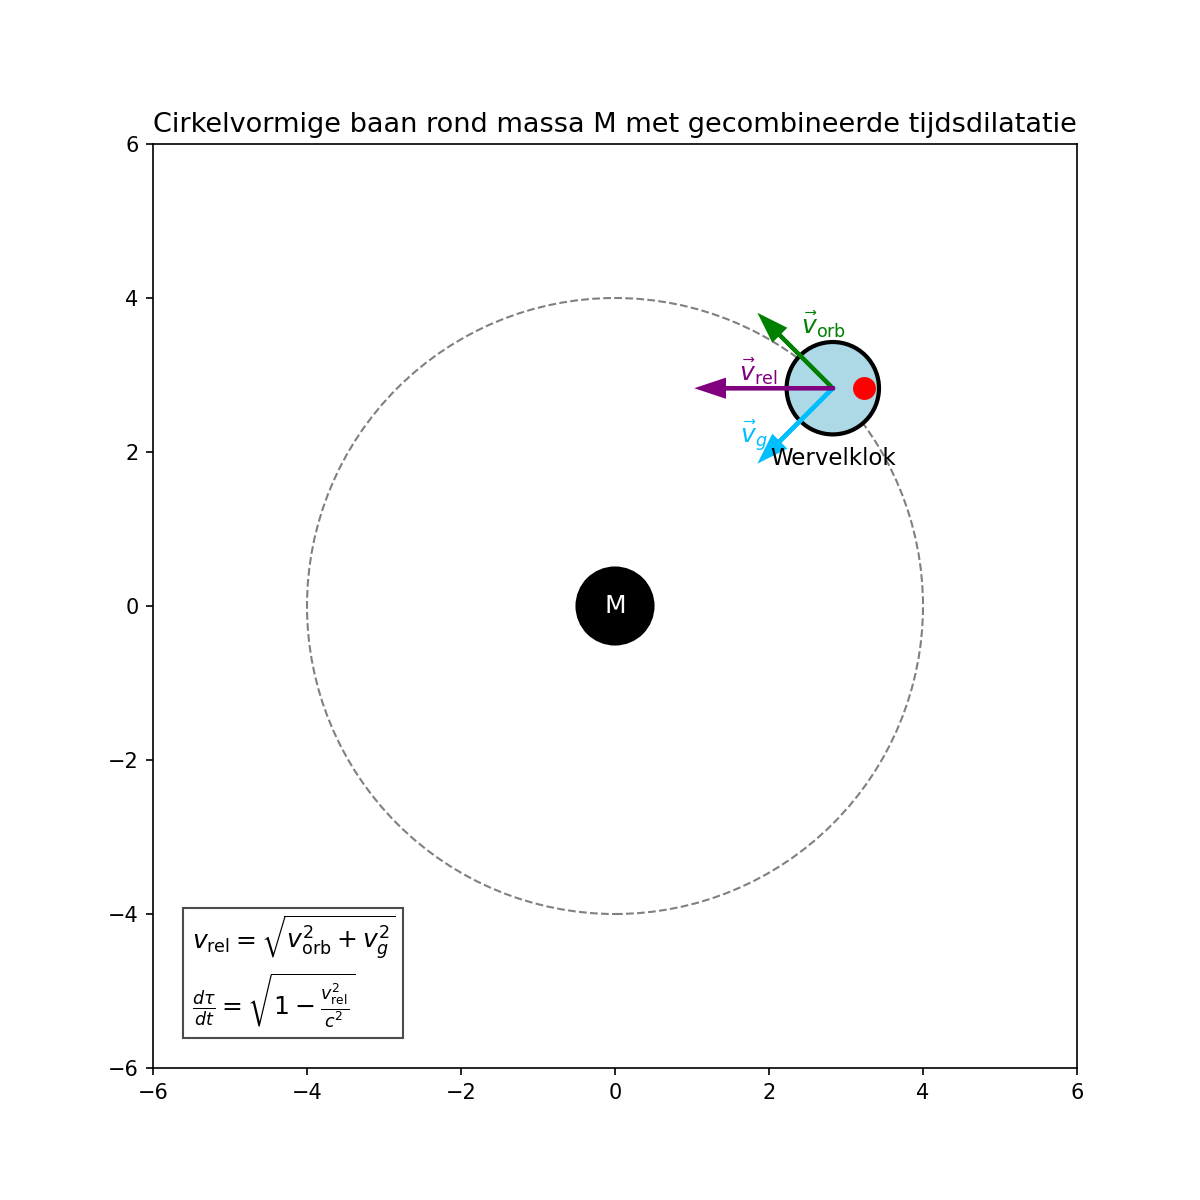
\includegraphics[width=0.85\textwidth]{08-BaanRondMassa}
    \caption{Een wervel in een cirkelvormige baan ervaart gecombineerde tijdsdilatatie door orbitaal- en ætherstroming. De klok ervaart zowel orbitale snelheid~$\vec{v}_{\mathrm{orb}}$ als ætherinstroom~$\vec{v}_g$, die samen resulteren in een gecombineerde relatieve snelheid~$\vec{v}_{\mathrm{rel}}$.}
    \label{fig:BaanRondMassa}
\end{figure}


De tijdsdilatatie wordt dus:
\[
    \frac{d\tau}{dt} = \sqrt{1 - \frac{3GM}{rc^2}}. \tag{6}
\]
Dit komt overeen met het exacte resultaat van Schwarzschild-geometrie voor cirkelvormige banen.

\begin{figure}[htbp]
    \centering
    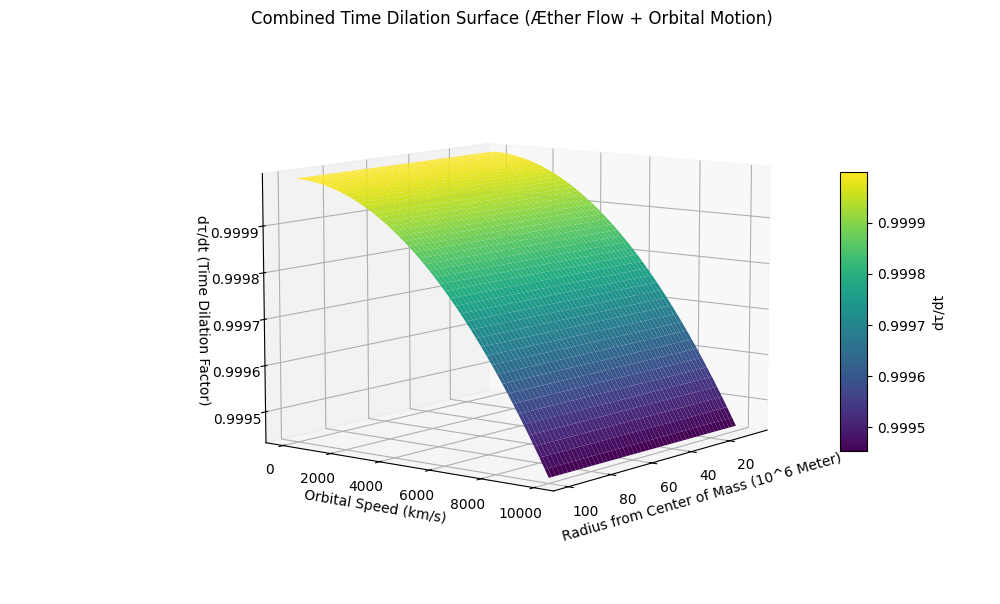
\includegraphics[width=0.85\textwidth]{/C:/Users/mr/IdeaProjects/VAM/TimeDialationCombined}
    \caption{Visuele representatie van de tijdsdilatatiefactor \( \frac{d\tau}{dt} \) als functie van zowel de orbitale snelheid \( v_{\text{orb}} \) als de gravitationele ætherinstroomsnelheid \( v_g \). Het oppervlak toont hoe beide bijdragen — inertiële en gravitatie-afgeleide ætherstroming — samen resulteren in een totale vertraging van de klok. De hyperbolische kromming van het oppervlak weerspiegelt de gecombineerde Lorentz- en Schwarzschild-dilatatie zoals beschreven in vergelijking (5) en (6).}
    \label{fig:TimeDialationCombined}
\end{figure}

\subsection*{Implicaties nabij een horizon}

Als $r \to r_s = 2GM/c^2$ nadert de instroomsnelheid $v_g(r)$ $c$ en vertraagt de klok van elke statische waarnemer tot nul. De ætherstroom onderdrukt de lokale wervelrotatie volledig, wat een natuurlijk mechanisme biedt voor het \("\)bevriezen van de tijd\("\) aan de gebeurtenishorizon.


\begin{figure}[htbp]
    \centering
    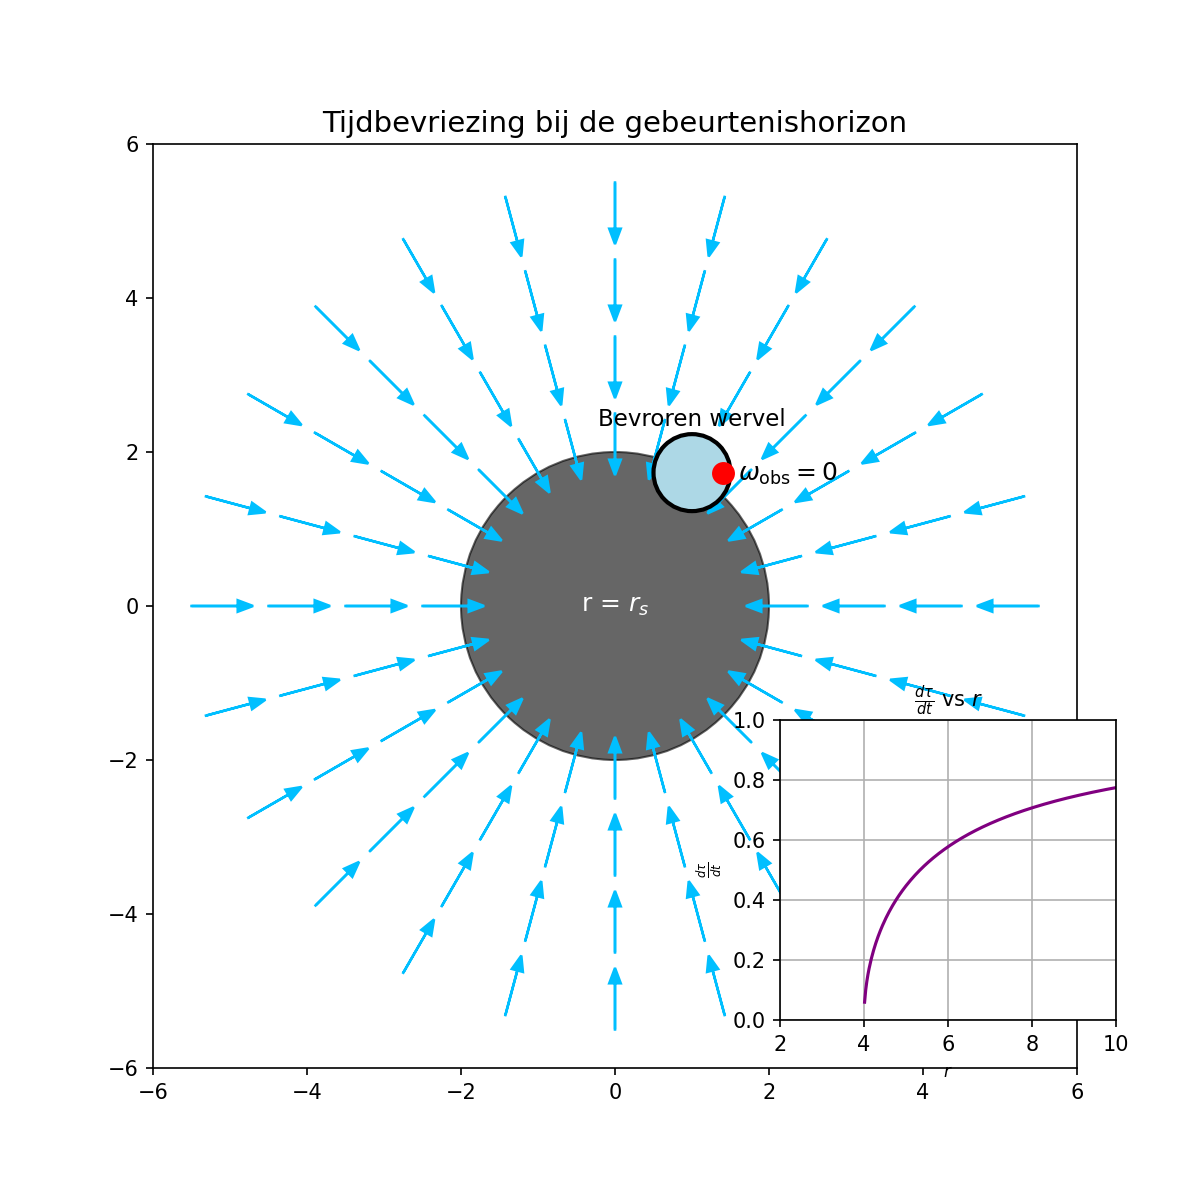
\includegraphics[width=0.85\textwidth]{10-HorizonTijdsbevriezing}
    \caption{Ætherstroming versnelt richting $r_s$, waar de waargenomen rotatie van de klok nul wordt. Bevriezing van tijd aan de gebeurtenishorizon $r = r_s$: de ætherstroming nadert~$c$, waardoor $\omega_{\mathrm{obs}} \to 0$. Rechts is de bijbehorende afname van $\frac{d\tau}{dt}$ als functie van afstand weergegeven.}
    \label{fig:HorizonTijdsbevriezing}
\end{figure}

\subsection*{Uniforme interpretatie}
\begin{figure}[htbp]
    \centering
    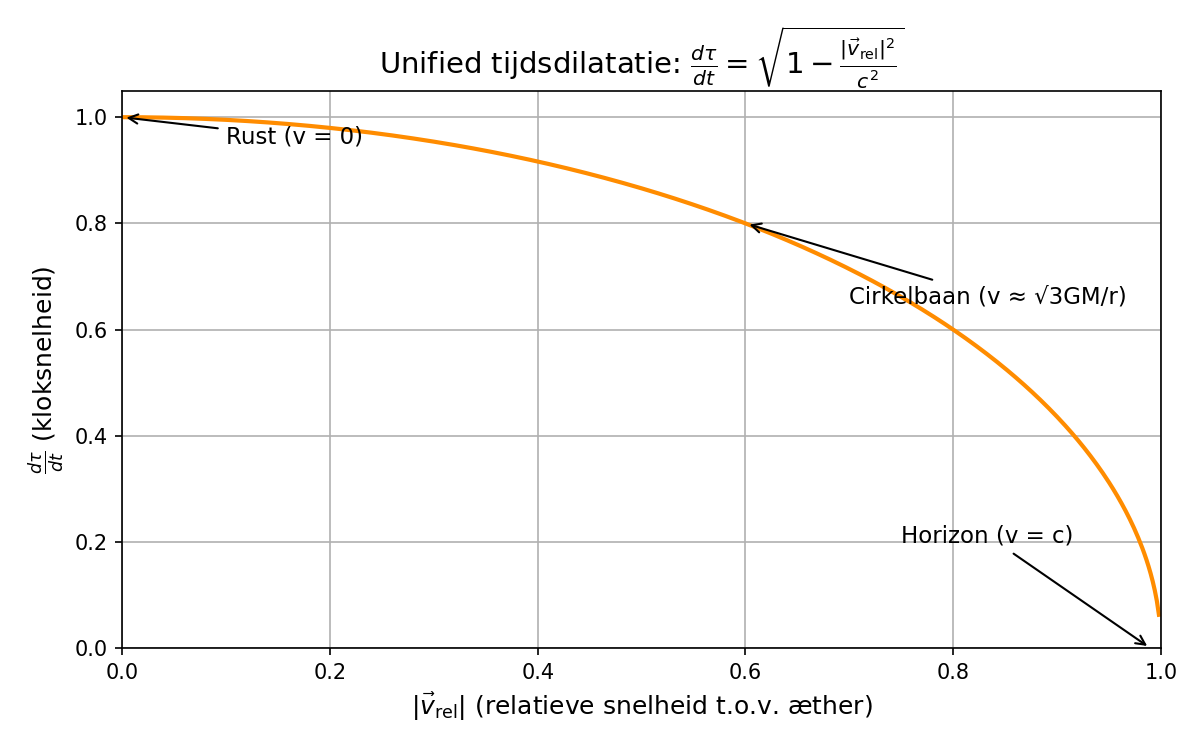
\includegraphics[width=0.85\textwidth]{11-TijdsvertragingRelatieveBeweging}
    \caption{Universele tijdsdilatatieformule in het Vortex Æther Model. De kloksnelheid daalt met toenemende relatieve snelheid~$|\vec{v}_{\mathrm{rel}}|$ ten opzichte van de æther. Bij $|\vec{v}_{\mathrm{rel}}| = c$ stopt de tijd.}
    \label{fig:TijdsvertragingRelatieveBeweging}
\end{figure}

Dit æthermodel maakt het mogelijk om alle relativistische tijdsdilatatie-effecten te zien als gevolgen van één principe:
\[
    \text{Kloksnelheidsreductie} \;\propto\; \text{relatieve beweging door æther}.
\]
Of deze relatieve beweging nu voortkomt uit traagheidssnelheid of uit ætherische instroom vanwege nabijgelegen massa, het waarneembare gevolg is hetzelfde. Daarom concluderen we:
\[
    \boxed{\frac{d\tau}{dt} = \sqrt{1 - \frac{|\vec{u} - \vec{v}_g|^2}{c^2}}}
\]
als de algemene tijdsdilatatieformule voor het Vortex Æther Model.

Voor mogelijke experimentele afwijkingen van deze tijdsdilatatieformules t.o.v. de algemene relativiteitstheorie, zie Appendix-B~\ref{appendix:AfwijkendeVoorspellingen}.
